\chapter{Program organization and compilation script}
\label{sc:info}
\index{Programming organization and compilation}

\label{loc:contenu} 

Currently the model is split between two directories: {\bf LMDZ.COMMON}
and {\bf LMDZ.MARS}. The reason for this separation is that all that
concerns the dynamics (and which is common to all planets) is in
{\bf LMDZ.COMMON} whereas all that concerns the Martian physics is
in {\bf LMDZ.MARS}. For historical reasons, {\bf LMDZ.MARS} still
includes a dynamical core, but it is strongly recommended to use
the {\bf LMDZ.COMMON} (mandatory if you want to run in parallel).

\noindent Here is a brief description of the contents of directory
{\bf LMDZ.COMMON}:
\begin{verbatim}
 libf/  model FORTRAN Source code (.F or .F90)
         and  include files (.h) organised in sub-directories
        (dynamics (dyn3d), filters (filtrez), interface with
         physical packages (dynphy_lonlat), ...)

 arch/  set of architecture files used by the makelmdz_fcm script

 makelmdz_fcm  script to use to compile the GCM and related
                utilities
 bin/ directory where executables generated by the makelmdz_fcm
       script will be generated

 ioipsl/ directory with scripts usefull to download and build the
          IOIPSL library (not needed by the Martian GCM).
\end{verbatim}

\noindent And a brief description of the
{\bf LMDZ.MARS} directory contents:
\begin{verbatim}
 libf/ Model FORTRAN Source code (.F or .F90)
        and  include files (.h) organised in sub-directories
        (physics (phymars), dynamics (dyn3d), filters (filtrez)...)

 deftank/ A collection of examples of parameter files required 
                to run the GCM (run.def, callphys.def, ...)
  
 util/ A set of programs useful for post-processing GCM outputs.

 makegcm (Obsolete) script that should be used to compile the GCM as well
            as related utilities (newstart, start2archive, testphys1d)
\end{verbatim}


\section{Organization of the model source files}
\index{Organization of the model source files}

The model source files are stored in various sub directories
in directories {\tt LMDZ.COMMON/libf} and {\tt LMDZ.MARS/libf}.
These sub-directories correspond to the different parts of the model: \\
In {\tt LMDZ.COMMON} one will find directories relevant for the dynamical core:
\begin{description}
\item{\bf grid:} mainly made up of "dimensions.h" file,
which contains the parameters that define the model grid,
i.e. the number of points in longitude (iim), latitude (jjm) and altitude
(llm).

\item{\bf dyn3d:} contains the dynamical core's serial code.

\item{\bf dyn3dpar:} contains the dynamical core's parallel code.

\item{\bf dy3d\_common:} contains routine common to serial and parallel dynamical cores.

\item{\bf dynphy\_lonlat:} contains the physics/dynamics interfaces, including in subdirectory
{\tt dynphy\_lonlat/phymars} the interface to the Martian physics.

\item{\bf filtrez:} contains the longitudinal filter sources applied in the
polar latitudes where the Courant-Friedrich-Levy stability criterion would otherwise be violated.

\item{\bf misc:} contains miscelaneous routines, neither specific to dynamics or physics.

\item{\bf phy\_common:} contains routines common to all physics packages (Mars, Venus, ...)

\item{\bf aeronomars, phymars:} these are links to the directories of the Mars physics package in
{\tt LMDZ.MARS/libf}

\item{\bf aeronostd, chimtitan, muphytitan, phystd, phytitan, phyvenus:} links, which may be broken, to
other physics packages (Titan, Venus, Generic GCM).
\end{description}

\noindent In {\tt LMDZ.MARS/libf} are subdirectories relevent to the Mars physics package:
\begin{description}
\item{\bf dyn3d, grid, filtrez:} Obsolete versions of the serial dynamical core (the
dynamics package included in LMDZ.COMMON should be used instead).

\item{\bf phymars:} contains the Martian physics routines.

\item{\bf aeronomars:} contains the Martian chemistry and thermosphere routines.
\end{description}

\section{Programming}

The model is written in {\bf Fortran}.
\begin{itemize}
\item The program sources are written in {\bf ``file.F"} 
or {\bf ``file.F90''} files.
The extension .F is the standard extension for fixed-form Fortran and
the extension .F90 is for free-form Fortran.
These files must be preprocessed (by a{\bf C preprocessor}
such as (cpp)) before compilation (this behaviour is, for most
compilers, implicitly obtained but using a capital F in the extention
of the file names).

\item Constants are placed in COMMON declarations,
located in the common ``include'' files {\bf "file.h"} or in relevant modules.

\item In general, variables should be passed from subroutine to subroutine
as arguments (and never as COMMON blocks).

\item In some parts of the code, for ``historical'' reasons,
the following rule is sometimes used: in the subroutine,
the variables (ex: \verb+name+) passed as an argument by the calling program
are given the prefix \verb+p+ (ex: \verb+pname+)
 while the local variables are given the prefix \verb+z+ (ex: \verb+zname+).
As a result, several variables change their prefix (and thus their name)
when passing from a calling subroutine to a called subroutine. 
\end{itemize}

\section{Model organization}
Figure~\ref{fg:organi_phys} describes the main subroutines called by physiq.F. 
\index{Model organization}
\begin{figure}
\begin{flushleft}
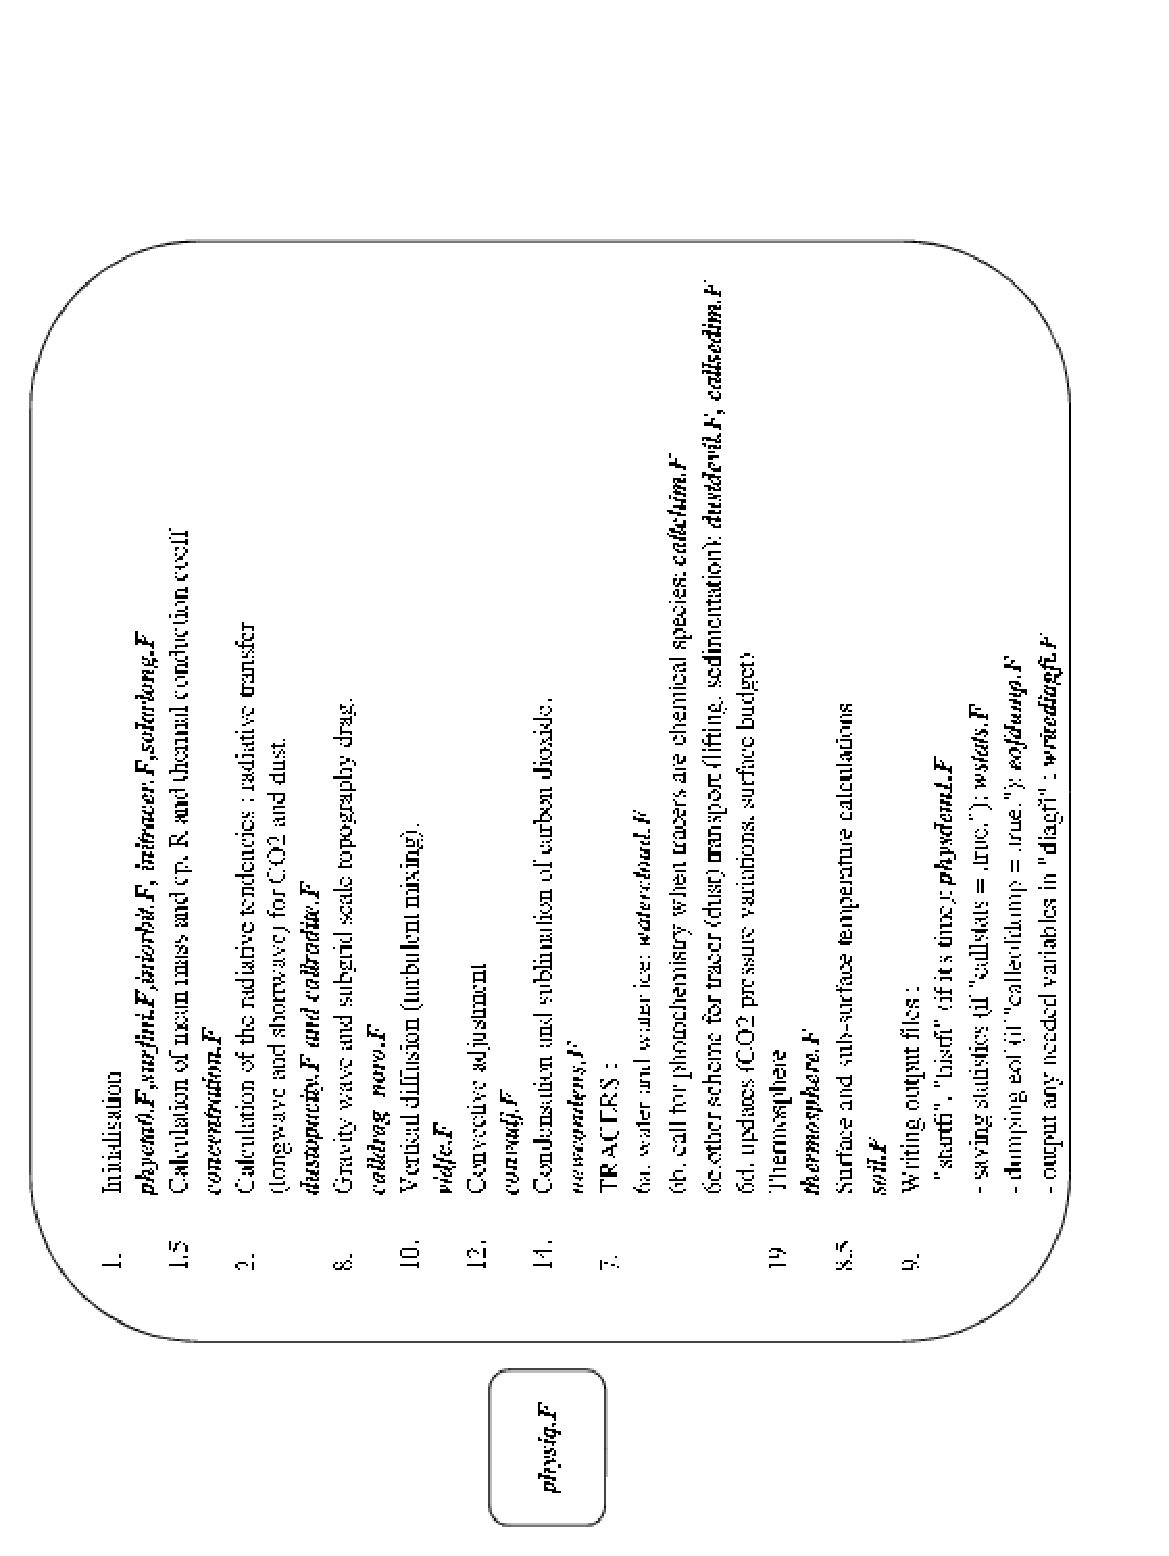
\includegraphics[scale=0.70,angle=-90]{Fig/physique.pdf}
\caption{Organigram of subroutine function physiq.F}
\label{fg:organi_phys}
\end{flushleft}
\end{figure}


%%%%%%%%%%%%%%%%%%%%%%%%%%%%%%%%%%%%%%%%%%%%%%%%%%
%  Compilation du modele
%%%%%%%%%%%%%%%%%%%%%%%%%%%%%%%%%%%%%%%%%%%%%%%%%%

\section{Compiling the model}
\index{Compiling the model}

\label{sc:compil1}
Technically, the model is compiled using the Unix utility {\tt make}.
The {\tt makelmdz\_fcm} utility script recreates the {\tt makefile} file
when necessary, for example, when a source file has been added or removed
since the last compilation.

\noindent {\bf None of this is visible to the user.
To (re-)compile the model just run the command}
\begin{verbatim}
makelmdz_fcm
\end{verbatim}
with adequate options (e.g.
{\tt makelmdz\_fcm -arch local -d 62x48x32 -p mars gcm}), as
described in section~\ref{sc:compile}.


\paragraph{Help manual for the makelmdz\_fcm script}
Use the "-h" option to learn about possible options:
\begin{verbatim}
makelmdz_fcm -h
\end{verbatim}
%%%%%%%%%%%%%%%%%%%%%%%%%%%%%%%%%%%%%%%%%%%%%%%%%%%%%%%
% makegcm.help:  lu dans makegcm
%%%%%%%%%%%%%%%%%%%%%%%%%%%%%%%%%%%%%%%%%%%%%%%%%%%%%%%
%{\footnotesize
\begin{verbatim}
makegcm [Options] prog


The makegcm script:
-------------------

1. compiles a series of subroutines located in the $LMDGCM/libf
 sub-directories.
 The objects are then stored in the libraries in $LIBOGCM.

2. then, makegcm compiles program prog.f located by default in
$LMDGCM/libf/dyn3d and makes the link with the libraries.

Environment Variables '$LMDGCM' and '$LIBOGCM'
 must be set as environment variables or directly
 in the makegcm file.

The makegcm command is used to control the different versions of the model
 in parallel, compiled using the compilation options 
 and the various dimensions, without having to recompile the whole model.

The FORTRAN libraries are stored in directory $LIBOGCM.


OPTIONS:
--------

The following options can either be defined by default by editing the
makegcm "script", or in interactive mode:

-d imxjmxlm  where im, jm, and lm are the number of longitudes,
             latitudes and vertical layers respectively.

-t ntrac   Selects the number of tracers present in the model

             Options -d and -t overwrite file 
             $LMDGCM/libf/grid/dimensions.h
             which contains the 3 dimensions of the
             horizontal grid 
             im, jm, lm plus the number of tracers passively advected
             by the dynamics ntrac,
             in 4 PARAMETER FORTRAN format 
             with a new file:
             $LMDGCM/libf/grid/dimension/dimensions.im.jm.lm.tntrac
             If the file does not exist already
             it is created by the script
             $LMDGCM/libf/grid/dimension/makdim

-p PHYS    Selects the set of physical parameterizations
           you want to compile the model with.
           The model is then compiled using the physical
           parameterization sources in directory:
            $LMDGCM/libf/phyPHYS

-g grille  Selects the grid type.
           This option overwrites file
           $LMDGCM/libf/grid/fxyprim.h
           with file
           $LMDGCM/libf/grid/fxy_grille.h
           the grid can take the following values:
           1. reg - the regular grid
           2. sin - to obtain equidistant points in terms of sin(latitude)
           3. new - to zoom into a part of the globe

-O "compilation options" set of fortran compilation options to use

-include path
           Used if the subroutines contain #include files (ccp) that 
           are located in directories that are not referenced by default.

-adjnt     Compiles the adjoint model to the dynamical code.

-filtre  filter
           To select the longitudinal filter in the polar regions.
           "filter" corresponds to the name of a directory located in
           $LMDGCM/libf. The standard filter for the model is "filtrez"
           which can be used for a regular grid and for a  
           grid with longitudinal zoom.

-link "-Ldir1 -lfile1 -Ldir2 -lfile2 ..."
           Adds a link to FORTRAN libraries
           libfile1.a, libfile2.a ... 
           located in directories dir1, dir2 ...respectively
           If dirn is a directory with an automatic path 
           (/usr/lib ... for example) 
           there is no need to specify  -Ldirn.

\end{verbatim}
}

%%%%%%%%%%%%%%%%%%%%%%%%%%%%%%%%%%%%%%%%%%%%%%%%%%%%%%%
